\section{Estructuras de datos}
\label{ch:implementacion:sec:estructurasDeDatos}

\subsection{CubeIndex}
\label{ch:implementacion:sec:CubeIndex}

Como se mencionó en \ref{subsec:marchingCubes:consideracionesGeometricas}, existen 256 formas posibles de atravesar un cubo con una superficie continua, que es lo mismo decir, existen 256 combinaciones posibles dados 8 vertices que pueden estar en 2 estados distintos (indicando que están dentro de una superficie cerrada o fuera de ésta)

Para poder identificar cada uno de estos 256 casos, se enumeran del 1 al 256 usando un arreglo de 8 bits, basándose en el estado de cada vértice usando la convención, por ejemplo, un cubo que tiene todos sus vértices marcados como fuera de la superficie (externos), tiene todos sus bits en cero, por lo tanto, el índice, desde ahora \emph{cubeIndex}, de este cubo es \hbox{$0_{10} = 0000 \; 0000_{2}$} (cero), de la misma manera, usando la convención, si un cubo sólo tiene el tercer vértice (vértice 2), dentro de la superficie, entonces, tiene su tercer bit en $1$ y el resto en cero, luego el \emph{cubeIndex} del cubo es $4_{10} = 0000 \; 0100_{2}$, si un cubo es atravesado por la mitad, dejando a la mitad de abajo dentro de la superficie, tiene los vértices 4, 5, 6 y 7 marcados como internos, por lo que los bits 4, 5, 6 y 7 (los ultimos 4), valen 1, por lo tanto, el \emph{cubeIndex} es $240_{10} = 1111 \; 0000_{2}$.

En general, el \emph{cubeIndex} se determina como se muestra en la figura \ref{f:ch:implementacion:sec:CubeIndex:cubeindex:cubeindex}, en este ejemplo el \emph{cubeIndex} tiene un valor de $9$.

\begin{figure}[hbt]
	\centering
	\fbox
	{
		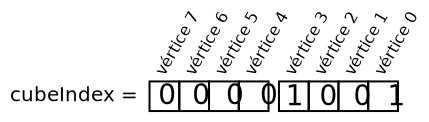
\includegraphics[width=0.8\textwidth]{images/implementacion/cubeindex.pdf}
	}
	\caption{Como se usan los vértices como bits ordenados para formar el \emph{cubeIndex}}
	\label{f:ch:implementacion:sec:CubeIndex:cubeindex:cubeindex}
\end{figure}

\subsection{edgeTable}
\label{ch:implementacion:sec:edgeTable}

Luego de establecer como identificar un cubo, es necesario poder conocer que aristas serian intersectadas por la superficie, para poder determinar un punto sobre estas aristas por las cuales se sostendrá un triángulo. Por ejemplo, si el vértice $0$, es el único vértice que queda dentro de la superficie, usando la convención, se puede asumir las aristas $0$, $3$ y $8$ serán aquellas las cuales la superficie intersectará al cubo.

Es por esto que se necesita una forma de relacionar un \emph{cubeIndex} con las aristas que serán atravesadas por la superficie.

Usando la misma estrategia que con el \emph{cubeindex} existen 4096 $(2^{12})$ combinaciones posibles de tomar 12 aristas que pueden intersectar a la superficie o no, por esto, cada caso, será identificado con un número de 12 bits, en el cual, cada bit representa a una arista, usando la convención como se muestra en la figura \ref{f:ch:implementacion:sec:CubeIndex:edgeTable:edge_convention}.

\begin{figure}[hbt]
	\centering
	\fbox
	{
		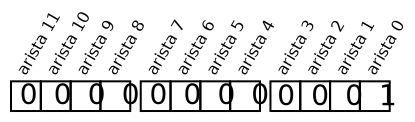
\includegraphics[width=0.8\textwidth]{images/implementacion/edgetable.pdf}
	}
	\caption{Convención para enumerar las 4096 combinaciones posibles de aristas}
	\label{f:ch:implementacion:sec:CubeIndex:edgeTable:edge_convention}
\end{figure}

La \emph{edgeTable} es un \emph{array} (arreglo) diseñado para asociar un \emph{cubeindex} con quellas aristas que son intersectadas. Este \emph{array} consta de 256 numeros (uno por cada caso o cada \emph{cubeindex}) de 12 bits, un bit para cada una de las 12 aristas del cubo en cuestión por las cuales pasa la superficie.

Para entender mejor, se supone el ejemplo de la figura \ref{f:ch:implementacion:sec:CubeIndex:edgeTable:example}.

\begin{figure}[hbt]
	\centering
	\fbox
	{
		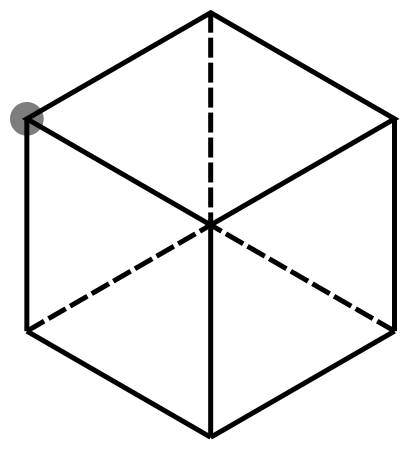
\includegraphics[width=0.3\textwidth]{images/implementacion/vertex_0.pdf}
	}
	\caption{Un cubo cuyo vértice $0$ es el único marcado.}
	\label{f:ch:implementacion:sec:CubeIndex:edgeTable:example}
\end{figure}

En este ejemplo, sólamente el vértice $0$, ha sido marcado como interno, luego, el \emph{cubeIndex} es $1_{10} = 0000 \; 0001_{2}$, dado esto, las aristas $0$, $3$ y $8$ serán eventualmente atravesadas por la superficie, por lo tanto:

\begin{quote}
	edgeTable[1] = 0x109
\end{quote}

Lo cual tiene un valor equivalente a: $109_{16} = 265_{10} = 0001 \; 0000 \; 1001_{2}$, lo que indica, viendo la notacion binaria, que las aristas $0$, $3$ y $8$ son las que serán atravesadas.

Otro ejemplo, se supone el caso de la figura \ref{f:ch:implementacion:sec:CubeIndex:edgeTable:example}

\begin{figure}[hbt]
	\centering
	\fbox
	{
		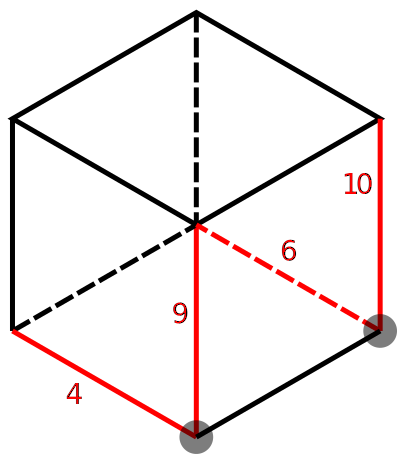
\includegraphics[width=0.3\textwidth]{images/implementacion/vertex_1.pdf}
	}
	\caption{Un cubo cuyos vértices $5$ y $6$ son los únicos marcados.}
	\label{f:ch:implementacion:sec:CubeIndex:edgeTable:example}
\end{figure}

En este caso, los vértices $5$ y $6$ han sido marcados como internos, luego, el \emph{cubeIndex} debe ser: $96_{10} = 0110 \; 0000_{2}$, por lo tanto la superficie deberia atravesar las aristas $4$, $9$, $6$ y $10$, para que asi, una superficie deje a estos vértices separados del resto.

Para saber que aristas finalmente son atravesadas, se debe consultar a la tabla \emph{edgeTable}, usando como índice, el \emph{cubeIndex} calculado anteriormente.

\begin{quote}
	edgeTable[96] = 0x650
\end{quote}

El valor entregado por la \emph{edgeTable} para el \emph{cubeIndex} $96$, es $0x650$ (hexadecimal), lo que es equivalente a:

\begin{quote}
	$650_{16} = 1616_{10} = 0110 \; 0101 \; 0000_{2}$
\end{quote}

Según la notación binaria, se puede ver que el valor entregado por la tabla \emph{edgeTable}, indica que los vértices $4$, $6$, $9$ y $10$ son aquellos que son atravesados por la superficie, de forma que los vertices $5$ y $6$ queden separados del resto.

\subsection{triTable}
\label{ch:implementacion:sec:triTable}

Una vez que se conocen aquellas aristas que seran atravesadas, es momento de crear la superficie interna que atraviese estas aristas y separe los vertices marcados de los demás. Para ello, es necesario poder generar aquellos triángulos que formen esta superficie.

La tabla \emph{triTable} es una tabla de 256 \emph{arrays} (arreglos) de 16 números cada uno, hay un arreglo por cada uno de los 256 casos descritos en \ref{ch:implementacion:sec:CubeIndex}, en cada caso, es necesario generar una serie de triángulos que describirán la superficie, y de todos los casos, como máximo se necesitan 5 triángulos para los casos mas complejos.

Analizando un caso simple, un cubo que solamente tiene un vértice marcado, necesita de sólo un triángulo que se sostenga de las aristas que convergen en ese vértice, para así crear una superficie que atraviese el cubo dejando a ese vértice separado del resto de los vértices del cubo, es por esto que el segundo elemento (\emph{cubeIndex} = 1) de la tabla \emph{triTable} tiene un valor:

\begin{quote}
	$triTable[1] = \{0, 8, 3, -1, -1, -1, -1, -1, -1, -1, -1, -1, -1, -1, -1, -1\}$
\end{quote}

Esto indica que el primer triángulo, es aquel que se sostiene (o corta) de las aristas: $0$, $8$ y $3$.

El resto de los $13$ números que quedan tienen un valor de $-1$, lo cual permite a cualquier implementacion del algoritmo, iterar en los números como tripletas, y detenerse cuando el primer número tenga un valor de $-1$.

De esta manera, cuando un cubo no tiene ninguno de sus vértices marcados (\emph{cubeIndex} = 0), o tiene todos sus vértices marcados (\emph{cubeIndex} = 255), los valores de la triTable para ambos casos son:

\begin{quote}
	$triTable[0]	= \{-1, -1, -1, -1, -1, -1, -1, -1, -1, -1, -1, -1, -1, -1, -1, -1\}$\\
	$triTable[255]	= \{-1, -1, -1, -1, -1, -1, -1, -1, -1, -1, -1, -1, -1, -1, -1, -1\}$
\end{quote}

Esto indica que para ambos casos, no se crea ningún trianglo, ya que cuando no tiene ningún vértice marcado indica que esta completamente fuera de la superficie, o en el otro caso, el cubo está contenido completamente dentro de la superficie, y ambos casos deben ser reemplazados por un cubo con cero triangulos.